\chapter{Lecture 12: Calculus (intro to derivatives)}

\subsection{Increasing and decreasing functions} \label{increasing decreasing 2}
In section \ref{one to one} we mentioned that functions which are everywhere increasing (or decreasing) are always one-to-one; in order to prove this fact we needed to use the definition of an increasing function. A function $f$ is increasing if, 

  	\bigskip
	
	\hfil\fbox{
	\begin{minipage}{0.5\columnwidth}{
	
	\vskip 0.1cm
	\begin{center}
	for all $a,b$ in the domain of $f$, whenever $b > a$, then $f(b) > f(a).$ 
	\end{center}
	}
	\end{minipage}}
	\bigskip
	\bigskip
	
\noindent On the other hand, $f$ is always decreasing if

  	\bigskip
	
	\hfil\fbox{
	\begin{minipage}{0.5\columnwidth}{
	
	\vskip 0.1cm
	\begin{center}
	for all $a,b$ in the domain of $f$, whenever $b > a$, then $f(b) < f(a).$ 
	\end{center}
	}
	\end{minipage}}
	\bigskip
	\bigskip
	
\subsection{Example} \label{ex12.0}
\begin{center}
\begin{tikzpicture}[yscale = 2.5,xscale=2]
	\draw[very thick, domain = -1.2:1.5, samples=200, smooth] plot (\x,{exp(-2*(\x+1))});
	\draw [gray, ->] (0,-0.2) -- (0,1.5) node [above left] {$f(x)$};
	\draw [gray, ->] (-1.4,0) -- (2.2,0) node [below right] {$x$};
	%\draw (2/3,0) node {$|$} node [above = 1mm] {$\alpha$};
\end{tikzpicture}
\end{center}
Is the above function increasing? \\

\noindent \textit{Solution:} \\
The function is decreasing (so it is not increasing).

\subsection{Example} \label{ex12.1}
\begin{center}
\begin{tikzpicture}[yscale = 2.5,xscale=2.7]
	\draw[very thick, domain = -0.8:1.5, samples=200, smooth] plot (\x,{\x*\x*(\x-1)});
	\draw [gray, ->] (0,-1.3) -- (0,1.5) node [above left] {$f(x)$};
	\draw [gray, ->] (-1.4,0) -- (2.2,0) node [below right] {$x$};
	\draw (2/3,0) node {$|$} node [above = 1mm] {$\alpha$};
\end{tikzpicture}
\end{center}
Above is the graph of the function $f(x) = x^2(x-1)$. What does $f$ do for
\begin{enumerate}
	\item $x < 0$
	\item $0 < x < \alpha$
	\item $x > \alpha$
\end{enumerate}
\noindent \textit{Solution:} \\
For $x < 0$, the function is increasing; for $0 < x < \alpha$ the function is decreasing; and for $x > \alpha$ the function is increasing.

\subsection{Rise over run (slope)} \label{slope}
In section \ref{secline} we introduced straight line functions as functions of the form $f(x) = mx + c$. The number $m$ is called the \textbf{slope} of the line because it tells us how \textit{steep} the line is (i.e., how quickly it rises or falls), and whether the line increases or decreases. In section \ref{secline} we plotted the graph of $f(x) = -2x + 4$, which has slope $m = -2$:
\begin{center}
	\begin{tikzpicture} [scale = 0.7]
	\draw (6,5) node {Graph of $f(x) = -2x + 4$.};
	\draw [fill = black] (0,0) circle (0.05cm) node [below left] {$(0,0)$};
	%\draw [dashed] (1,2) -- (1,-0.1) node [below] {$1$};
	%\draw [dashed] (1,2) -- (-0.1,2) node [left] {$2$};
	\draw [->] (-1,0) -- (5,0) node [below right] {$x$};
	\draw (3,-2) -- (-1,6) node [above left] {$f(x)$};
	\draw [->] (0,-1) -- (0,5.5) node [above left] {$y$};
	%\draw [fill = black] (1,2) circle (0.08cm) node [above right] {$(1,2)$};
	%\draw [fill = black] (0,4) circle (0.08cm) node [above right] {$(0,4)$};
	\draw (1,0) node {$|$} node  [below = 1mm] {$1$};
	\draw (0.1,4) -- (-0.1,4) node [left] {$4$};
	\draw (0.1,2) -- (-0.1,2) node [left] {$2$};
	\draw [ultra thick, dashed] (0,2) -- (1,2);
	\draw [ultra thick, dashed] (0,2) -- (0,4);
	\end{tikzpicture}
\end{center}
By looking at the dashed lines on the above graph of $f(x)$ (and comparing them to the triangle below), you should be able to see that $f(x)$ decreases by $2$ whenever $x$ increases by $1$. Hence $f(x)$ is a decreasing function (you are encouraged to check that $f(x)$ formally satisfies the definition of an decreasing function).
\begin{center}
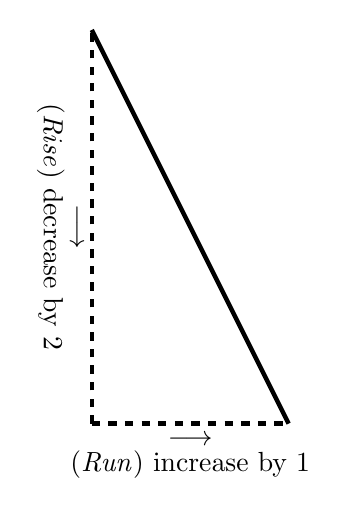
\begin{tikzpicture}[scale = 2.5]
	\draw [ultra thick, dashed] (0,2) -- (1,2) node [midway, below] {$\longrightarrow$} node [midway, below = 2mm] {(\textit{Run}) increase by $1$};
	\draw [ultra thick, dashed] (0,2) -- (0,4) node [rotate = -90,  midway, below] {$\longrightarrow$} node [rotate = -90, midway, below = 2mm] {(\textit{Rise}) decrease by $2$};
	\draw [ultra thick] (0,4) -- (1,2);
\end{tikzpicture}
\end{center} \label{rise over run}
On the above diagram of the triangle, we have labelled the vertical segment ``\textbf{rise},'' and we have labelled the horizontal segment ``\textbf{run},'' so that for the line $f(x) = -2x + 4$ we have
\[
\textbf{rise} = -2  \qquad \text{and} \qquad  \textbf{run} = 1.
\]
In general, the slope, $m$, of any straight line is given by

  	\bigskip
	
	\hfil\fbox{
	\begin{minipage}{0.15\columnwidth}{
	
	%\vskip 0.05cm
	\begin{center}
	$m =\displaystyle{\frac{\text{rise}}{\text{run}}}$
	\end{center}
	}
	\end{minipage}}
	\bigskip
	\bigskip

\noindent Below is the graph of the function $g(x) = 3x + 1$ which has $m = 3$. 
\begin{center}
	\begin{tikzpicture} [scale = 0.7]
	\draw[domain = -1.2:2.3, samples=200, smooth] plot (\x,{3*\x+1});
	\draw (6,5) node {Graph of $g(x) = 3x + 1$.};
	\draw [fill = black] (0,0) circle (0.05cm) node [below left] {$(0,0)$};
	\draw [->] (-1,0) -- (5,0) node [below right] {$x$};
	\draw [->] (0,-1) -- (0,8) node [above left] {$y$};
	\draw (1,0) node {$|$} node  [below = 1mm] {$1$};
	\draw (0.1,4) -- (-0.1,4) node [left] {$4$};
	\draw (0.1,7) -- (-0.1,7) node [left] {$7$};
	\draw (2,0) node {$|$} node [below = 1mm] {$2$};
	\draw [ultra thick, dashed] (1,4) -- (2,4);
	\draw [ultra thick, dashed] (2,4) -- (2,7);
	\end{tikzpicture}
\end{center}
By looking at the graph of $g(x)$ you should be able to tell that $g(x)$ increases by 3 whenever $x$ increases by 1. That is, $g(x)$ has a rise of 3 corresponding to a run of $1$. So, $m = \frac{\text{rise}}{\text{run}} = \frac{3}{1} = 3.$ Hence $g(x)$ is an increasing function. \\

\subsection{Example}
Try to answer the following questions before looking at the solutions.
\begin{enumerate}
\item When $m > 0$ does a straight line increase or decrease?
\item When $m < 0$ does a straight line increase or decrease?
\item Does larger $|m|$ correspond to a steeper or flatter slope?
\item When $m = 0$ is the line vertical or horizontal? 
\end{enumerate}
\bigskip
\noindent \textit{Solution:} \\
(1) increase. (2) decrease. (3) steeper. (4) horizontal. 


\section{Rate of change and the definition of derivative} \label{rate of change}
\noindent Another way to talk about the slope of $g(x)$ from section \ref{slope} is to say that ``the \textbf{rate of change} of $g(x)$, with respect to $x$, is $3$.'' This means that whenever $x$ increases by some real number, $a$, the result is that $g(x)$ increases by the amount $3a$. So if $x$ increases by 1 then $g(x)$ increases by $3$, and if $x$ increases by $0.5$ then $g(x)$ increases by $3\times0.5 = 1.5$. Using this terminology to describe $f(x) = -2x + 4$ we would say that ``the rate of change of $f(x)$, with respect to $x$, is $-2$. The rate of change of a straight line function (i.e., a function of the form $f(x) = mx + c$) is given by $m$.\\

\noindent It is easy to find the rate of change (i.e., slope) of a straight line function from its graph, or from its formula (we have just done this for $f(x)$ and $g(x)$); this is partly because the rate of change of a straight line is \textit{constant}. However, there are an infinite amount of interesting functions that do not have a constant rate of change. All functions whose graphs are curved have a non-constant rate of change. \\

\noindent The graphs in examples \ref{ex12.0} and \ref{ex12.1} are both of functions that have non-constant rates of change; their rates of change depends on which position along the $x$-axis that we are focusing on. That is, these functions have slopes that depend on $x$. \\

\noindent Below are two copies of a graph of the function $k(x) = \e^{-2x}$. Two triangles have been drawn, one on each copy, which closely approximate the slope of $k(x)$ along the interval at which they are drawn; one is drawn on the interval $[a,b]$ and the other is drawn on the interval $[c,d]$.
\begin{center}
	\begin{minipage}{0.3\textwidth}
	\begin{center}
	\begin{tikzpicture}[scale = 2]
		\draw[domain = -0.2:1.5, samples=200, smooth] plot (\x,{exp(-2*(\x))});
		\draw [gray, ->] (0,-0.2) -- (0,1.5) node [above left] {$k(x)$};
		\draw [gray, ->] (-0.4,0) -- (1.8,0) node [below right] {$x$};
		\draw (0.1,0) node {\tiny{$|$}} node [below = 2mm] {$a$};
		\draw (0.5,0) node {\tiny{$|$}} node [below = 1mm] {$b$};
		\draw [fill = black] (0.1,{exp(-2*(0.1))}) circle (0.03cm);
		\draw [fill = black] (0.5,{exp(-2*(0.5))}) circle (0.03cm);
		\draw [ultra thick, dashed] (0.1,{exp(-2*(0.1))}) -- (0.5,{exp(-2*(0.5))});
		\draw [ultra thick, dashed] (0.5,{exp(-2*(0.5))})  --  (0.1,{exp(-2*(0.5))});
		\draw [ultra thick, dashed] (0.1,{exp(-2*(0.5))}) -- (0.1,{exp(-2*(0.1))});
		%\draw (2/3,0) node {$|$} node [above = 1mm] {$\alpha$};
	\end{tikzpicture}
	\end{center}
	\end{minipage}%
	\begin{minipage}{0.5\textwidth}
	\begin{center}
	\begin{tikzpicture}[scale = 2]
		\draw[domain = -0.2:1.5, samples=200, smooth] plot (\x,{exp(-2*(\x))});
		\draw [gray, ->] (0,-0.2) -- (0,1.5) node [above left] {$k(x)$};
		\draw [gray, ->] (-0.4,0) -- (1.8,0) node [below right] {$x$};
		\draw (0.8,0) node {\tiny{$|$}} node [below = 2mm] {$c$};
		\draw (1.2,0) node {\tiny{$|$}} node [below = 1mm] {$d$};
		\draw [fill = black] (0.8,{exp(-2*(0.8))}) circle (0.03cm);
		\draw [fill = black] (1.2,{exp(-2*(1.2))}) circle (0.03cm);
		\draw [ultra thick, dashed] (0.8,{exp(-2*(0.8))})  -- (1.2,{exp(-2*(1.2))});
		\draw [ultra thick, dashed] (1.2,{exp(-2*(1.2))})  --  (0.8,{exp(-2*(1.2))});
		\draw [ultra thick, dashed] (0.8,{exp(-2*(1.2))}) -- (0.8,{exp(-2*(0.8))});
		%\draw (2/3,0) node {$|$} node [above = 1mm] {$\alpha$};
	\end{tikzpicture}
	\end{center}
	\end{minipage}
\end{center} 
The (steeper) slope represented by the triangle on the left is that of the straight line that goes through the point $(a,h(a))$, and the point $(b,h(b))$. Similarly, the (flatter) slope represented by the triangle on the right is that of the straight line that goes through the point $(c,h(c))$, and the point $(d,h(d))$. \label{average roc} \\

\noindent In each case, the slopes represented by these triangles tell us the \textbf{average rate of change} of the function $k$, for the intervals that the triangles are on. \label{instantaneous roc} \\

\noindent Looking at the triangle on the left, the distance, \textbf{run}, along the $x$-axis (along the interval $[a,b]$) is \textbf{run}$ = b - a$. The distance, \textbf{rise}, along the $y$-axis (along the interval $[k(a),k(b)]$) is given by \textbf{rise} $ = k(b) - k(a)$. So, the average rate of change of $k(x)$ on the interval $[a,b]$ is given by \label{avg slope}
 
  	\bigskip
	
	\hfil\fbox{
	\begin{minipage}{0.4\columnwidth}{
	
	%\vskip 0.05cm
	\begin{center}
	$\text{avg slope} =\displaystyle{\frac{\text{rise}}{\text{run}}} = \frac{k(b) - k(a)}{b - a}$.
	\end{center}
	}
	\end{minipage}}
	\bigskip
	\bigskip


\noindent The \textit{exact} rate of change of $k$, with respect to $x$, at any given point along the $x$ axis, is called the \textbf{instantaneous rate of change}. Finding a sensible definition for this idea (the exact rate of change of a function at any given single point) is somewhat tricky. So far, we only really understand slopes to belong to lines, which are defined using at least two separate points; now we need to define a slope that belongs to a single point (hence the term ``instantaneous''). The following diagrams demonstrate what happens when we take the average rate of change over successively smaller and smaller intervals. The diagrams depict the average rate of change of $k$ on the interval $[a,a + h_i],$ where $h_i$ is a positive real number. We let $i \in \set{1,2,3,4}$ with $h_4 < h_3 < h_2 < h_1$. The dashed lines pass through the points $(a,k(a))$ and $(a+h_i,k(a+h_i))$.
\begin{center}
	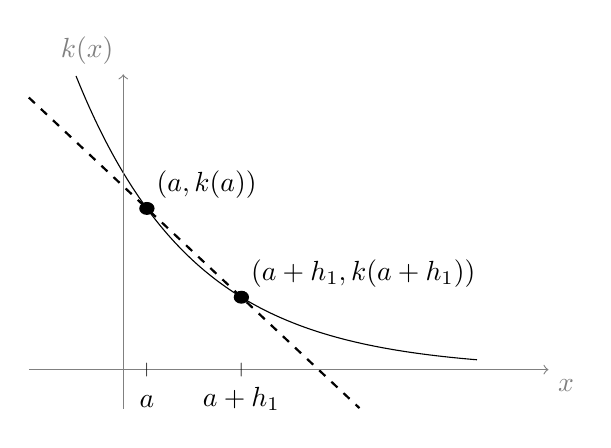
\begin{tikzpicture}[yscale = 2.5, xscale = 3]
		\draw[domain = -0.2:1.5, samples=200, smooth] plot (\x,{exp(-2*(\x))});
		\draw[dashed, thick, domain = -0.4:1, samples=200, smooth] plot (\x,{0.931444 - 1.12713*\x});
		\draw [gray, ->] (0,-0.2) -- (0,1.5) node [above left] {$k(x)$};
		\draw [gray, ->] (-0.4,0) -- (1.8,0) node [below right] {$x$};
		\draw (0.1,0) node {\tiny{$|$}} node [below = 2mm] {$a$};
		\draw (0.5,0) node {\tiny{$|$}} node [below = 1mm] {$a + h_1$};
		\draw [fill = black] (0.1,{exp(-2*(0.1))}) circle (0.03cm) node [above right] {$(a,k(a))$};
		\draw [fill = black] (0.5,{exp(-2*(0.5))}) circle (0.03cm) node [above right] {$(a+h_1,k(a+h_1))$};;
%		\draw [ultra thick, dashed] (0.1,{exp(-2*(0.1))}) -- (0.5,{exp(-2*(0.5))});
%		\draw [ultra thick, dashed] (0.5,{exp(-2*(0.5))})  --  (0.1,{exp(-2*(0.5))});
%		\draw [ultra thick, dashed] (0.1,{exp(-2*(0.5))}) -- (0.1,{exp(-2*(0.1))});
		%\draw (2/3,0) node {$|$} node [above = 1mm] {$\alpha$};
	\end{tikzpicture}
\end{center}
\begin{center}
	\begin{tikzpicture}[yscale = 2.5, xscale = 3]
		\draw[domain = -0.2:1.5, samples=200, smooth] plot (\x,{exp(-2*(\x))});
		\draw[dashed, thick, domain = -0.3:0.8, samples=200, smooth] plot (\x,{0.95369 - 1.3496*\x});
		\draw [gray, ->] (0,-0.2) -- (0,1.5) node [above left] {$k(x)$};
		\draw [gray, ->] (-0.4,0) -- (1.8,0) node [below right] {$x$};
		\draw (0.1,0) node {\tiny{$|$}} node [below = 2mm] {$a$};
		\draw (0.5,0) node [below = 1mm] {$a + h_2$};
		\draw (0.3,0) node {\tiny{$|$}};
		\draw [fill = black] (0.1,{exp(-2*(0.1))}) circle (0.03cm);
		\draw [fill = black] (0.3,{exp(-2*(0.3))}) circle (0.03cm);
%		\draw [ultra thick, dashed] (0.1,{exp(-2*(0.1))}) -- (0.5,{exp(-2*(0.5))});
%		\draw [ultra thick, dashed] (0.5,{exp(-2*(0.5))})  --  (0.1,{exp(-2*(0.5))});
%		\draw [ultra thick, dashed] (0.1,{exp(-2*(0.5))}) -- (0.1,{exp(-2*(0.1))});
		%\draw (2/3,0) node {$|$} node [above = 1mm] {$\alpha$};
	\end{tikzpicture}
\end{center}
\begin{center}
	\begin{tikzpicture}[yscale = 2.5, xscale = 3]
		\draw[domain = -0.2:1.5, samples=200, smooth] plot (\x,{exp(-2*(\x))});
		\draw[dashed, thick, domain = -0.3:0.8, samples=200, smooth] plot (\x,{0.974556 - 1.55825*\x});
		\draw [gray, ->] (0,-0.2) -- (0,1.5) node [above left] {$k(x)$};
		\draw [gray, ->] (-0.4,0) -- (1.8,0) node [below right] {$x$};
		\draw (0.1,0) node {\tiny{$|$}} node [below = 2mm] {$a$};
		\draw (0.35,0) node [below = 1mm] {$a + h_3$};
		\draw (0.15,0) node {\tiny{$|$}};
		\draw [fill = black] (0.1,{exp(-2*(0.1))}) circle (0.03cm);
		\draw [fill = black] (0.15,{exp(-2*(0.15))}) circle (0.03cm);
%		\draw [ultra thick, dashed] (0.1,{exp(-2*(0.1))}) -- (0.5,{exp(-2*(0.5))});
%		\draw [ultra thick, dashed] (0.5,{exp(-2*(0.5))})  --  (0.1,{exp(-2*(0.5))});
%		\draw [ultra thick, dashed] (0.1,{exp(-2*(0.5))}) -- (0.1,{exp(-2*(0.1))});
		%\draw (2/3,0) node {$|$} node [above = 1mm] {$\alpha$};
	\end{tikzpicture}
\end{center}
\begin{center}
	\begin{tikzpicture}[yscale = 2.5, xscale = 3]
		\draw[domain = -0.2:1.5, samples=200, smooth] plot (\x,{exp(-2*(\x))});
		\draw[dashed, thick, domain = -0.3:0.8, samples=200, smooth] plot (\x,{0.982461 - 1.6373*\x});
		\draw [gray, ->] (0,-0.2) -- (0,1.5) node [above left] {$k(x)$};
		\draw [gray, ->] (-0.4,0) -- (1.8,0) node [below right] {$x$};
		\draw (0.1,0) node {\tiny{$|$}} node [below = 2mm] {$a$};
		\draw (0.35,0) node [below = 1mm] {$a + h_4$};
		\draw (0.1001,0) node {\tiny{$|$}};
		\draw [fill = black] (0.1,{exp(-2*(0.1))}) circle (0.03cm);
		\draw [fill = black] (0.1001,{exp(-2*(0.1001))}) circle (0.03cm);
%		\draw [ultra thick, dashed] (0.1,{exp(-2*(0.1))}) -- (0.5,{exp(-2*(0.5))});
%		\draw [ultra thick, dashed] (0.5,{exp(-2*(0.5))})  --  (0.1,{exp(-2*(0.5))});
%		\draw [ultra thick, dashed] (0.1,{exp(-2*(0.5))}) -- (0.1,{exp(-2*(0.1))});
		%\draw (2/3,0) node {$|$} node [above = 1mm] {$\alpha$};
	\end{tikzpicture}
\end{center}
In the final diagram we used $h_4 = 0.001$, so the interval $[a,a+h_4]$ has length $a + h_4 - a = h_4 = 0.001.$ As the interval $[a,a+h_i]$ gets smaller and smaller, the two points, $(a,k(a))$ and $(a + h_i,k(a + h_i))$, become so close together that they become approximately the same point. The smaller the interval gets (i.e., the smaller $h_i$ gets), the more accurate this approximation becomes. Hence, in the limit as the interval becomes infinitely small, the approximation becomes exact. We define the instantaneous rate of change of $k(x)$ at the point $x = a$ to be the average rate of change of $k(x)$ over an infinitely small interval, i.e., for $[a,a+h],$ as $h \rightarrow 0$. \\

\noindent Recall that the average rate of change of $k(x)$, on the interval $[a,a+h]$, is the slope of the line through the points $(a,k(a))$ and $(a+h,k(a+h))$. Using the result in the box on page \pageref{avg slope}, this slope is given by
\[
\text{avg slope} = \frac{\text{rise}}{\text{run}} = \frac{k(a+h) - k(a)}{(a + h) - a} = \frac{k(a+h) - k(a)}{h}.
\]
By the definition of instantaneous rate of change, it follows that the instantaneous rate of change of $k(x)$, at the point $a$, is given by letting $h \rightarrow 0$, i.e., 
\[
\lim_{h \rightarrow 0}\brac{\frac{k(a+h) - k(a)}{h}}
\]
In general, for any point, $x$, it follows that the instantaneous rate of change of $k(x)$, with respect to $x$, is given by the same formula (just replacing $a$ with $x$). We call this the \textbf{dervative of $\boldsymbol{k(x)}$ with respect to $\boldsymbol{x}$}. We write $\frac{d}{dx}\brac{k(x)}$, where the expression ``$\frac{d}{dx}$'' means ``the derivative with respect to $x$.'' So,  \label{derivative}

  	\bigskip
	
	\hfil\fbox{
	\begin{minipage}{0.45\columnwidth}{
	
	%\vskip 0.05cm
	\begin{center}
	$\displaystyle{\frac{d}{dx}\brac{k(x)} = \lim_{h \rightarrow 0}\brac{\frac{k(x+h) - k(x)}{h}}}$
	\end{center}
	}
	\end{minipage}}
	\bigskip
	\bigskip
	
\noindent Sometimes we write $k'(x)$ instead of $\frac{d}{dx}\brac{k(x)},$ and we say ``$k$ dash $x$'' for short; both of these notations mean the same thing. The act of finding the derivative is called \textbf{differentiation}. \label{differentiation} \\


\subsection{Formulas for finding derivatives} \label{derivative formulas}
As we will soon see, calculating this limit (i.e., using the definition of the derivative) can become arduous. To make life easier, most mathematicians use formulas that help them calculate derivatives without having to carefully find this limit each time. In this section we will introduce the most important of these formulas. In this course you wont be required to calculate derivatives using the definition of the derivative, instead you will use the handy formulas that we introduce here. If you wanted, you could skip all references to the definition of a derivative, and just practice using the formulas (since the definition of a derivative is not strictly covered in this course).

\subsubsection{Powers}
We will now introduce a formula for quickly finding the derivatives of power functions, i.e., functions of the form $f(x) = x^k$, where $k \neq 0$. \\

\noindent The formula is (for all real numbers $k \neq 0$),

  	\bigskip
	
	\hfil\fbox{
	\begin{minipage}{0.45\columnwidth}{
	
	%\vskip 0.05cm
	\begin{center}
	$f(x) = x^k \;\; \text{implies} \;\; f'(x) = kx^{k-1}$
	\end{center}
	}
	\end{minipage}}
	\bigskip
	\bigskip
	
\noindent When $k = 0$ we have $x^k = x^0 = 1$ which is a constant, so we use the formula for the drivative of a constant, which we will look at after we are done with this. \\

\noindent Instead of giving the full proof, we will only prove two cases, $k = 2$ and $k=3$; the reason we do this is because the full proof is much easier once we know formulas for the derivative of a logarithm and the derivative of an exponential function, which we will introduce later. \\ 

\noindent Let $f(x) = x^2$. Using the definition of a derivative from section \ref{rate of change} we have
\begin{align*}
f'(x)  & = \lim_{h \rightarrow 0}\brac{\frac{f(x+h) - f(x)}{h}} \\
	& = \lim_{h \rightarrow 0}\brac{\frac{(x+h)^2 - x^2}{h}} \tag{since $f(x) = x^2$} \\
	& = \lim_{h \rightarrow 0}\brac{\frac{x^2 + 2xh + h^2 - x^2}{h}} \tag{expanding the brackets} \\
	& = \lim_{h \rightarrow 0}\brac{\frac{2xh + h^2}{h}} \\
	& = \lim_{h \rightarrow 0}\brac{\frac{2xh/h + h^2/h}{h/h}} \tag{dividing top and bottom by $h$} \\
	& = \lim_{h \rightarrow 0}\brac{\frac{2x + h}{1}} \tag{cancelling common factors of $h$} \\
	& = 2x. \tag{since $h \rightarrow 0$}
\end{align*}
So the derivative of $x^2$ is $2x$. \\

\noindent Let $g(x) = x^3$. Using the definition of a derivative from section \ref{rate of change} we have
\begin{align*}
f'(x)  & = \lim_{h \rightarrow 0}\brac{\frac{g(x+h) - g(x)}{h}} \\
	& = \lim_{h \rightarrow 0}\brac{\frac{(x+h)^3 - x^3}{h}} \tag{since $g(x) = x^3$} \\
	& = \lim_{h \rightarrow 0}\brac{\frac{x^3 + 3x^2h + 3xh^2 + h^3 - x^3}{h}} \tag{expanding the brackets} \\
	& = \lim_{h \rightarrow 0}\brac{\frac{3x^2h + 3xh^2 + h^3}{h}} \\
	& = \lim_{h \rightarrow 0}\brac{\frac{3x^2h/h + 3xh^2/h + h^3/h}{h/h}} \tag{dividing top and bottom by $h$} \\
	& = \lim_{h \rightarrow 0}\brac{\frac{3x^2 + 3xh + h^2}{1}} \tag{cancelling common factors of $h$} \\
	& = 3x^2. \tag{since $h \rightarrow 0$}
\end{align*}
So the derivative of $x^3$ is $3x^2$. \\

\noindent Using the formula in the box, we have $\frac{d}{dx}\brac{x^2} = 2x^{2-1} = 2x$ and we also have $\frac{d}{dx}\brac{x^3} = 3x^{3-1} = 3x^2.$ So, in both cases the formula in the box agrees with the results that we just obtained using the definition of a derivative.

\subsubsection{Constants}
The formula for the derivative of a constant is perhaps the easiest to use. If a function, $f$, is constant, i.e., if $f(x) = c$ for some real number, $c$, then what is the rate of change of $f$ with respect to $x$? The answer is zero, because $f(x)$ is constant, so it does not change. \\

\noindent Hence the formula is

  	\bigskip
	
	\hfil\fbox{
	\begin{minipage}{0.45\columnwidth}{
	
	%\vskip 0.05cm
	\begin{center}
	$f(x) = c \;\; \text{implies} \;\; f'(x) = 0$
	\end{center}
	}
	\end{minipage}}
	\bigskip
	\bigskip
	
\noindent The proof of this one is straight forward; using the definition of a derivative we have
\begin{align*}
f'(x)  & = \lim_{h \rightarrow 0}\brac{\frac{f(x+h) - f(x)}{h}} \\
	& = \lim_{h \rightarrow 0}\brac{\frac{c - c}{h}} \tag{since $f(x) = c$} \\
	& = \lim_{h \rightarrow 0}\brac{0} \tag{since $c-c = 0$} \\
	& = 0.
\end{align*}

\subsubsection{Sums} \label{linear derivatives}
Suppose we have a function $f(x) = g(x) + k(x)$, where $g$ and $k$ are two arbitrary functions whose derivatives both exist (some functions do not have derivatives, which is something that we will look at in section \ref{not have derivatives}). So, $f(x)$ is a sum of two other functions. \\

\noindent Examples of functions that $f(x)$ might be, include 
\begin{itemize}
\item $f(x) = mx + c$, which is a sum of $g(x) = mx$ and $k(x) = c$. 
\item $f(x) = ax^2 + bx + c$, which is a sum of $g(x) = ax^2$ and $k(x) = bx + c$ (notice that $bx+c$ is a function which itself is also a sum of two functions).
\item $f(x) = e^{x^2} - \ln(2x)$, which is a sum of $g(x) = e^{x^2}$ and $k(x) = -\ln(2x)$.
\item $f(x) = \displaystyle{\frac{x^2 + x}{12}}$ which is a sum of $g(x) = \frac{x^2}{12}$ and $k(x) = \frac{x}{12}.$ 
\end{itemize}

\noindent Then the derivative of $f(x)$ is given by the formula

  	\bigskip
	
	\hfil\fbox{
	\begin{minipage}{0.6\columnwidth}{
	
	%\vskip 0.05cm
	\begin{center}
	$f(x) = g(x) + k(x) \;\; \text{implies} \;\; f'(x) = g'(x) + k'(x)$
	\end{center}
	}
	\end{minipage}}
	\bigskip
	\bigskip

\noindent This formula says that, if a function is a sum of some separate terms, then we can break down the task of finding the derivative of the function, into the task of finding the derivatives of its individual terms.\\

\noindent In the $\frac{d}{dx}$ notation we would express this formula as
\[
\frac{d}{dx}\brac{g(x) + k(x)} = \frac{d}{dx}\brac{g(x)} + \frac{d}{dx}\brac{k(x)}.
\]

\noindent This property is called a \textbf{linearity} property of differentiation. We spoke about linearity properties in section \ref{linearity}, when we were learning about summation notation. In that section we learned that there are two linearity properties (go back and read section \ref{linearity} again if you do not remember what these two properties are). \label{linearity (differentiation)} \\

\subsubsection{Constant multiples}
We just learned that differentiation has a linearity property; i.e., we learned that taking the derivative of a sum of two functions is the same as taking the sum of the individual derivatives of those functions. We will now see that differentiation has the other linearity property that we spoke about in section \ref{linearity}. \\

\noindent Let $f(x) = cg(x)$, where $c$ is some real number constant. So, $f(x)$ is equal to some function, $g(x)$, multiplied by a constant, $c$. Then 

  	\bigskip
	
	\hfil\fbox{
	\begin{minipage}{0.6\columnwidth}{
	
	%\vskip 0.05cm
	\begin{center}
	$f(x) = cg(x) \;\; \text{implies} \;\; f'(x) = cg'(x)$
	\end{center}
	}
	\end{minipage}}
	\bigskip
	\bigskip

\noindent In the $\frac{d}{dx}$ notation we would express this formula as
\[
\frac{d}{dx}\brac{cg(x)} = c\frac{d}{dx}\brac{g(x)}.
\]
Notice that we can ``pull the constant outside'' the brackets, and just differentiate the function $g(x)$. \\


\noindent To convince yourself that this is the second linearity property, you are encouraged to compare this formula to the linarity properties of summation notation in section \ref{linearity}. To indicate that differentiation has both linearity properties, we can refer to differentiation as a \textbf{linear operator}, or say that differentiation is \textbf{linear}. \label{linear operator}  

\subsubsection{Proof of sums and constant multiples formulas}
Let $f(x) = g(x) + k(x)$ for some functions $g$ and $k$. Using the definition of a derivative, we have
\begin{align*}
f'(x) 	& = \lim_{h \rightarrow 0}\brac{\frac{f(x+h) - f(x)}{h}} \\
	& = \lim_{h \rightarrow 0}\brac{\frac{g(x+h) + k(x+h) - g(x) - k(x)}{h}} \tag{since $f(x) = g(x) + k(x)$} \\
	& = \lim_{h \rightarrow 0}\brac{\frac{g(x+h) - g(x) + k(x+h) - k(x)}{h}} \tag{rearranging terms} \\
	& = \lim_{h \rightarrow 0}\brac{\frac{g(x+h) - g(x)}{h} + \frac{k(x+h) - k(x)}{h}} \tag{algebra of fractions} \\
	& =  \lim_{h \rightarrow 0}\brac{\frac{g(x+h) - g(x)}{h}} + \lim_{h \rightarrow 0}\brac{\frac{k(x+h) - k(x)}{h}} \tag{limits are also linear} \\
	& = g'(x) + k'(x). \tag{by the definition of a derivative}
\end{align*} 
So $f'(x) = g'(x) + k'(x),$ as required. \\

\noindent Now, let $f(x) = cg(x)$ for some real constant $c$, and some function $g$. Using the definition of a derivative, we have
\begin{align*}
f'(x) 	& = \lim_{h \rightarrow 0}\brac{\frac{f(x+h) - f(x)}{h}} \\
	& = \lim_{h \rightarrow 0}\brac{\frac{cg(x+h) - cg(x)}{h}} \tag{since $f(x) = cg(x)$} \\
	& = \lim_{h \rightarrow 0}\brac{c\frac{g(x+h) - g(x)}{h}} \\
	& = c\lim_{h \rightarrow 0}\brac{\frac{g(x+h) - g(x)}{h}} \tag{limits are also linear} \\
	& = cg'(x). \tag{by the definition of a derivative}
\end{align*}
So $f'(x) = cg'(x),$ as required. \\

\noindent We have proved that both of the linearity properties hold for differentiation, but in both cases we used the fact that taking the limit is also a linear operator. This fact was first mentioned in section \ref{linearity}. To prove that taking a limit is linear, we would need a more accurate and detailed understanding of limits, which is usually taught in a subject on mathematical analysis.

\subsection{Example}
Using the formulas that we just introduced, we are able to find the derivatives of a huge variety of functions.  \\

\noindent Using the power functions, constants, sums, and constant multiples formulas, differentiate $f(x) = 7x - 2x^3 + 6 - \frac{1}{x}$, where $x > 0$. \\

\noindent \textit{Solution:} \\
Using the sums formula we have
\[
\frac{d}{dx}\brac{7x - 2x^3 + 6 - \frac{1}{x}} = \frac{d}{dx}\brac{7x} + \frac{d}{dx}\brac{-2x^3} + \frac{d}{dx}\brac{6} + \frac{d}{dx}\brac{-\frac{1}{x}}. 
\]
Using the constant multiples formula, the right hand side becomes
\[
7\frac{d}{dx}\brac{x} - 2\frac{d}{dx}\brac{x^3} + \frac{d}{dx}\brac{6} - \frac{d}{dx}\brac{\frac{1}{x}}.
\]
Using the formula for the derivative of a constant we have $\frac{d}{dx}\brac{6} = 0$, so this expression becomes
\[
7\frac{d}{dx}\brac{x} - 2\frac{d}{dx}\brac{x^3} - \frac{d}{dx}\brac{\frac{1}{x}}.
\]
If we rewrite these terms as powers we will see where we can use the power function fomula. We have $x = x^1$, and $\frac{1}{x} = x^{-1}$ (using index laws). So, we can rewrite this expression as
\[
7\frac{d}{dx}\brac{x^1} - 2\frac{d}{dx}\brac{x^3} - \frac{d}{dx}\brac{x^{-1}}.
\]
So after all this we have
\[
\frac{d}{dx}\brac{7x - 2x^3 + 6 - \frac{1}{x}} = 7\frac{d}{dx}\brac{x^1} - 2\frac{d}{dx}\brac{x^3} - \frac{d}{dx}\brac{x^{-1}}.
\]
Using the formula for the derivative of a power function, we get
\begin{align*}
7\frac{d}{dx}\brac{x^1} - 2\frac{d}{dx}\brac{x^3} - \frac{d}{dx}\brac{x^{-1}} & = 7\times1x^{1-1} - 2\times3x^{3-1} - (-1)x^{-1-1} \\
	& = 7x^0 - 6x^2 +x^{-2} \\
	& = 7 - 6x^2 + x^{-2} \tag{since $x^0 = 1$} \\
	& = 7 - 6x^2 + \frac{1}{x^2}. \tag{index laws}
\end{align*}
So putting this together we have
\[
\frac{d}{dx}\brac{7x - 2x^3 + 6 - \frac{1}{x}} = 7 - 6x^2 + \frac{1}{x^2}.
\]

In section \ref{not have derivatives} you will see why we required $x > 0$.

\subsection{Example}
Differentiate the following:
\begin{enumerate}
\item $x^3 + x - 17$
\item $(3x)^2$
\item $\frac{1}{\sqrt{x}}$ where $x > 0$. 
\end{enumerate}
\bigskip

\noindent \textit{Solution to (1):} \\
We have
\begin{align*}
\frac{d}{dx}\brac{x^3 + x - 17} & = \frac{d}{dx}\brac{x^3} + \frac{d}{dx}\brac{x} + \frac{d}{dx}\brac{-17} \tag{sum formula} \\
	& = 3x^{3-1} + 1\times x^{1-1} + \frac{d}{dx}\brac{-17} \tag{power function formula} \\
	& = 3x^2 + 1 + \frac{d}{dx}\brac{-17} \tag{since $x^0 = 1$} \\
	& = 3x^2 + 1. \tag{constants formula}
\end{align*}
\bigskip

\noindent \textit{Solution to (2):} \\
We have
\begin{align*}
\frac{d}{dx}\brac{(3x)^2} & = \frac{d}{dx}\brac{3^2x^2} \tag{index laws} \\
		& =  \frac{d}{dx}\brac{9x^2} \\
		& = 9\times2x^{2-1} \tag{power function formula} \\
		& = 18x^1 \\
		& = 18x.
\end{align*}
\bigskip

\noindent \textit{Solution to (3):} \\
We have
\begin{align*}
\frac{d}{dx}\brac{\frac{1}{\sqrt{x}}} & = \frac{d}{dx}\brac{\frac{1}{x^{1/2}}} \tag{since $\sqrt{x} = x^{1/2}$ (see section \ref{fractional indices})} \\
		& = \frac{d}{dx}\brac{\brac{x^{1/2}}^{-1}} \tag{index laws} \\
		& = \frac{d}{dx}\brac{x^{-1/2}} \tag{index laws} \\
		& = -\frac{1}{2}x^{-1/2-1} \tag{power function formula} \\
		& = -\frac{1}{2}x^{-3/2}. \tag{since $-1/2 - 1 = -1/2 - 2/2 = \frac{-1-2}{2} = \frac{-3}{2}$}
\end{align*}

In the next section you will see why we had to specify that $x > 0$.

\subsection{Existence of derivatives} \label{not have derivatives}
Previously we mentioned that some functions do not have derivatives. Can you come up with some examples? \\

\subsubsection{Continuity}
In section \ref{continuity and discontinuity}, we learned about continuity and discontinuity of functions. The function $f(x) = \frac{1}{x}$ is not continuous at $x = 0$ (because it is not defined there) so its derivative is not defined there either. Functions which are discontinuous do not have derivatives, unless they are restricted to a domain on which they are continuous. If we restrict $f(x) = \frac{1}{x}$ to the domain $x > 0$ (or to the domain $x < 0$), then this function does have a derivative. \\

\noindent As another example, the function $f(x) = \sqrt{x}$ does not have a derivative when $x \in \R$; to take the derivative we need to restrict the domain of this function to $x \geq 0$, so that the function is defined everywhere.


\subsubsection{Smoothness}
Aside from being continuous, functions also need to be ``smooth'' to have a derivative. That is, their graphs need to be straight or curvy; they cannot have sharp spikes or corners. All of the continuous functions that we have graphed in this subject so far have been smooth. Below are graphs of two functions, $f(x)$ and $g(x)$, which are not smooth.  \\

\noindent This function, $f(x) = |x|$, is not differentiable at $x = 0,$ 
\begin{center}
	\begin{tikzpicture}[yscale = 2.5, xscale = 3]
		\draw[very thick, domain = 0:1, samples=200, smooth] plot (\x,{\x}) node [above right] {$f(x) = |x|$};
		\draw[very thick, domain = -1:0, samples=200, smooth] plot (\x,{-\x});
		\draw [gray, ->] (0,-0.2) -- (0,1.3) node [above left] {$y$};
		\draw [gray, ->] (-1.3,0) -- (1.3,0) node [below right] {$x$};
	\end{tikzpicture}
\end{center}
\bigskip


\noindent This function, $g(x)$, is not differentiable at the point $x = 1,$
\begin{center}
	\begin{tikzpicture}[yscale = 2.5, xscale = 2.5]
		\draw[very thick, domain = -0.5:1, samples=200, smooth] plot (\x,{\x*\x});
		\draw[very thick, domain = 1:1.5, samples=200, smooth] plot (\x,{\x}) node [right] {$\scases{g(x)}{x^2}{\text{if} \; x < 1}{x}{\text{if} \; x \geq 1}$};
		\draw [gray, ->] (0,-0.2) -- (0,1.5) node [above left] {$y$};
		\draw [gray, ->] (-0.5,0) -- (1.8,0) node [below right] {$x$};
		\draw (1,0) node {\tiny{$|$}} node [below = 1mm] {$1$};
		\draw (0.05,1) -- (-0.05,1) node [left] {$1$};
	\end{tikzpicture}
\end{center}
\bigskip 


\noindent To see why $f(x) = |x|$ is not differentiable at $x = 0$, we can look at the definition of a derivative. We have
\begin{align*}
f'(0) & = \lim_{h \rightarrow 0}\brac{\frac{f(0+h) - f(0)}{h}} \\
	& = \lim_{h \rightarrow 0}\brac{\frac{|0+h| - |0|}{h}} \tag{since $f(x) = |x|$} \\
	& = \lim_{h \rightarrow 0}\brac{\frac{|h|}{h}} \tag{since $|0| = 0$}.
\end{align*}
This limit does not exist! Hence $f'(0)$ does not exist. To see why this limit does not exist, we need to take a careful look at the definition of the absolute value function. The definition of the absolute value function is
\[
\scases{|h|}{h}{\text{if} \; h \geq 0}{-h}{\text{if} \; h < 0}
\]
So this means that
\[
\frac{|h|}{h} = \frac{h}{h} = 1, \;\; \text{when $h > 0$}.
\]
and
\[
\frac{|h|}{h} = \frac{-h}{h} = -1, \;\; \text{when $h < 0$}.
\]
Now, let's think about the definition of a limit. What does it mean when we claim that $\displaystyle{\lim_{h \rightarrow 0}}\bfrac{|h|}{h} = \ell$, for some number $\ell$?\\

\noindent It means that we can obtain a number arbitrarily close to $\ell$, just by letting the distance from $h$ to zero become small enough. However, $h$ does not have to be positive; we could choose a negative value for $h$, say $-0.0001$; when we decide to choose only negative values for $h$ we get, for example,
\[
h = -0.0001 \;\;\; \text{implies} \;\;\; \frac{|h|}{h} = \frac{-(-0.0001)}{(-0.0001)} = -1,
\]
and
\[
h = -0.000001 \;\;\; \text{implies} \;\;\; \frac{|h|}{h} = \frac{-(-0.000001)}{(-0.000001)} = -1,
\]
and so on, for smaller and smaller choices of $h$. Thus, if we only looked at negative values of $h$, then we would become convinced that as $h \rightarrow 0$, $\frac{|h|}{h} \rightarrow -1$. On the other hand, if we only looked at positive values for $h$ we would find that $\frac{|h|}{h} = 1$; for example,
\[
h = 0.0001 \;\; \text{implies} \;\;\; \frac{|h|}{h} = \frac{0.0001}{0.0001} = 1.
\]
So, our choice for the number $\ell$ depends on our choice for $h$ (being negative or positive). \\

\noindent That is,
\[
\lim_{h\rightarrow 0}\bfrac{|h|}{h} = 1, \;\;\;\; \text{when $h$ approaches from the positive side of $0$.}
\]
and
\[
\lim_{h \rightarrow 0}\bfrac{|h|}{h} = -1 \;\;\;\; \text{when $h$ approaches from the negative side of $0$.}
\]
So there is no unique choice for $\ell$, and hence we say that the limit does not exist. \\

\noindent If we used a similar approach to look at the function $g(x)$, then we would find that $g(x)$ does not have a derivative at $x = 1$, for the same reason (no unique choice for the limit). \\

\noindent In fact, any functions that are not smooth will run into the same problem. \\

\noindent In relating the idea of ``smoothness'' to the definition of a derivative, we had to wave our hands around a lot, so you might not be feeling completely satisfied; if this is the case, then you are encouraged to study mathematical analysis, since ideas like this become easy to understand (and far easier to explain) once you have learned the proper definition of a limit.

\section{More formulas for finding derivatives} \label{more derivative formulas}

\subsection{Exponential function} \label{derivative of exponential}
The nicest derivative of all is the derivative of the exponential function, $f(x) = e^x$. After 
reading this section on the exponential function, you might want to go and have a look at the end of appendix \ref{appendix B}, where we talk about ``compound interest, natural growth, and the number $\e$.'' The remarkable fact that we will prove here is that $\e^x$ is \textit{its own rate of change} with respect to $x$. That is,
 
  	\bigskip
	
	\hfil\fbox{
	\begin{minipage}{0.4\columnwidth}{
	
	%\vskip 0.05cm
	\begin{center}
	$f(x) = \e^x \;\; \text{implies} \;\; f'(x) = \e^x$
	\end{center}
	}
	\end{minipage}}
	\bigskip
	\bigskip

\noindent We could also rewrite this as
\[
\frac{d}{dx}\brac{\e^x} = \e^x.
\]

\noindent In lecture 16 (section \ref{chain rule}), we will learn about the ``chain rule,'' which will make the following fact more obvious. However, we need to introduce this fact a little early: In general, for any real constant, $a$, we have
 
  	\bigskip
	
	\hfil\fbox{
	\begin{minipage}{0.4\columnwidth}{
	
	%\vskip 0.05cm
	\begin{center}
	$f(x) = \e^{ax} \;\; \text{implies} \;\; f'(x) = a\e^{ax}$
	\end{center}
	}
	\end{minipage}}
	\bigskip
	\bigskip

\noindent In order to prove that $\frac{d}{dx}\brac{\e^x} = \e^x$, we can use the definition of a derivative. Let $f(x) = \e^x$, then
\begin{align*}
f'(x)  & = \lim_{h \rightarrow 0}\brac{\frac{f(x + h) - f(x)}{h}} \tag{definition of a derivative} \\
	& = \lim_{h \rightarrow 0}\brac{\frac{\e^{x + h} - \e^x}{h}} \tag{since $f(x) = \e^x$}\\
	& = \lim_{h \rightarrow 0}\brac{\frac{\e^{x}\e^{h} - \e^x}{h}} \tag{index laws} \\
	& = \lim_{h \rightarrow 0}\brac{\frac{\e^{x}\brac{\e^{h} - 1}}{h}} \tag{factorising} \\
	& = \e^{x}\lim_{h \rightarrow 0}\brac{\frac{\e^{h} - 1}{h}} \tag{limits are linear, see section \ref{linearity}}
\end{align*}
In the last step we treated $\e^x$ as a constant, because we are taking a limit with respect to $h$, not $x$. Now, we need to prove that
\[
\lim_{h \rightarrow 0}\brac{\frac{\e^{h} - 1}{h}} = 1.
\]
To do this, we can use the power series representation of $\e^x$ that we introduced in section \ref{power series} (go back and have a look now if you don't rememeber). First we will use some algebra,
\[
\lim_{h \rightarrow 0}\brac{\frac{\e^{h} - 1}{h}} = \lim_{h \rightarrow 0}\brac{\frac{1}{h}\brac{\e^{h} - 1}} 
\]
Now, replacing $\e^h$ with its power series representation,
\begin{align*}
\lim_{h \rightarrow 0}\brac{\frac{1}{h}\brac{\e^{h} - 1}} & = \lim_{h \rightarrow 0}\brac{\frac{1}{h}\brac{1 + h + \frac{h^2}{2!} +  \frac{h^3}{3!} + \ldots  - 1}} \\
		& = \lim_{h \rightarrow 0}\brac{\frac{1}{h}\brac{h + \frac{h^2}{2!} +  \frac{h^3}{3!} + \ldots}} \tag{since $1-1 = 0$} \\
		& =  \lim_{h \rightarrow 0}\brac{\frac{h}{h} + \frac{h^2}{h2!} +  \frac{h^3}{h3!} + \ldots} \\
		& = \lim_{h \rightarrow 0}\brac{1 + \frac{h}{2!} +  \frac{h^2}{3!} + \ldots} \tag{cancelling common factors of $h$}
\end{align*}
Now, as $h \rightarrow 0$, all of the terms except $1$ will go to zero, since they all have a power of $h$ in the numerator. Hence
\[
 \lim_{h \rightarrow 0}\brac{1 + \frac{h}{2!} +  \frac{h^2}{3!} + \ldots} = 1.
\]
Which is what we wanted to show. It follows that
\[
\e^{x}\lim_{h \rightarrow 0}\brac{\frac{\e^{h} - 1}{h}} = \e^x \times 1 = \e^x.
\]
Hence $f'(x) = \e^x$, as required.

\subsection{Example}  \label{ex12.101}
Differentiate $f(x) = 7\e^x + \e^{7x} + \e^{7-x}$. \\

\noindent \textit{Solution:} \\
We have,
\begin{align*}
\frac{d}{dx}\brac{7\e^x + \e^{7x} + \e^{7-x}} & = \frac{d}{dx}\brac{7\e^x + \e^{7x} + \e^{7}\e^{-x}} \tag{index laws} \bsk
& =  7\frac{d}{dx}\brac{\e^x} + \frac{d}{dx}\brac{\e^{7x}} + \e^7\frac{d}{dx}\brac{\e^{-x}} \tag{linearity} \bsk
	& = 7\e^x + 7\e^{7x} - \e^7\e^{-x}. \tag{derivative of $\e^{ax}$} \ssk
	& = 7\e^x + 7\e^{7x} - \e^{7-x}. \tag{index laws}
\end{align*}

\subsection{Logarithm function} \label{log no proof}
We now give the derivative of the logarithm function with base $\e$, i.e., $f(x) = \ln(x)$ (the natural log). Recall that the domain of this function is $x > 0$ (see section \ref{symblog} for revision). 

  	\bigskip
	
	\hfil\fbox{
	\begin{minipage}{0.45\columnwidth}{
	
	%\vskip 0.05cm
	\begin{center}
	$f(x) = \ln(x) \;\; \text{implies} \;\; f'(x) = \frac{1}{x}$, $\;\;\;\;\;\;\; \text{where $x > 0$}$
	\end{center}
	}
	\end{minipage}}
	\bigskip
	\bigskip

\noindent We could rewrite this as
\[
\frac{d}{dx}\brac{\ln(x)} = \frac{1}{x}.
\]
Since $x > 0$, we know that the slope of the logarithm function is always positive (so it is always increasing). We also know that $\frac{1}{x}$ grows as $x \rightarrow 0$; so the slope gets greater (i.e., steeper) as we get closer to $x = 0$. Similarly, as we get further from $0$, i.e., as $x \rightarrow \infty$, the expression $\frac{1}{x}$ gets smaller; thus the slope gets flatter as $x$ gets larger. We should be able to see all of this manifested in the graph of the natural log function below:
\begin{center}
	\begin{tikzpicture}[scale = 2]
		\draw[thick, domain = 0.2:2.5, samples=200, smooth] plot (\x,{ln(\x)}) node [right] {$f(x) = \ln(x)$};
		\draw [gray, ->] (0,-1.4) -- (0,1) node [above left] {$f(x)$};
		\draw [gray, ->] (-0.4,0) -- (2.5,0) node [below right] {$x$};
		\draw (1,0) node {\tiny{$|$}} node [below = 1mm] {$1$};
		\draw (1,-1.5) node [rotate = -25] {$\longleftarrow$};
		\draw (1,-1.6) node [right = 4mm] {slope gets steeper}; 
		\draw (2.4,0.5) node [rotate = -25] {$\longleftarrow$};
		\draw (2.4,0.4) node [right = 4mm] {slope gets flatter}; 
		%\draw (2/3,0) node {$|$} node [above = 1mm] {$\alpha$};
	\end{tikzpicture}
\end{center}
The formula for the derivative of the natural log is proved at the end of section \ref{right-to-left substitution}, once we have learned about antiderivatives (i.e., integrals), and some integration techniques. \\

\noindent When differentiating expressions that involve logarithms, you will often need to recall the logarithm laws, from section \ref{log laws}.

\subsection{Example}
Differentiate $f(x) = \ln(4x) + \ln\brac{x^4}$, where $x > 0$. \\

\noindent \textit{Solution:} \\
We have,
\begin{align*}
\frac{d}{dx}\brac{\ln(4x) + \ln\brac{x^4}} & = \frac{d}{dx}\brac{\ln(4) + \ln(x) + \ln(x^4)}  \tag{log law (L1), see section \ref{log laws}} \\
	& = \frac{d}{dx}\brac{\ln(4) + \ln(x) + 4\ln(x)} \tag{log law (L2)} \\
	& = \frac{d}{dx}\brac{\ln(4)} + \frac{d}{dx}\brac{\ln(x)} + 4\frac{d}{dx}\brac{\ln(x)} \tag{linearity} \\
	& = 0 + \frac{d}{dx}\brac{\ln(x)} + 4\frac{d}{dx}\brac{\ln(x)} \tag{derivative of a constant} \\
	& = \frac{1}{x} + \frac{4}{x} \tag{derivative of natural log} \\
	& = \frac{5}{x}.
\end{align*}

\section{Application of derivatives: turning points} \label{turning points}
Sometimes we might need to find the maximum (or minimum) height of a function; we will actually need to do this often in the later parts of this course in order to determine the \textit{mode} of continuous distributions (we will learn about the mode in section \ref{mode definition}). \\

\noindent Consider the following graph,
\begin{center}
	\begin{tikzpicture}[yscale = 3, xscale = 2]
		\draw[very thick, domain = -0.6:1.4, samples=200, smooth] plot (\x,{\x*\x*(\x - 1)}) node [right] {$f(x) = x^2(x-1)$};
		\draw [gray, ->] (0,-0.8) -- (0,1) node [above left] {$f(x)$};
		\draw [gray, ->] (-0.7,0) -- (1.5,0) node [below right] {$x$};
		\draw (2/3,0) node {\tiny{$|$}} node [above] {$\alpha$};
		%\draw (2/3,0) node {$|$} node [above = 1mm] {$\alpha$};
	\end{tikzpicture}
\end{center}
What is the slope of $f(x)$ at the origin? The function is neither increasing nor decreasing at the origin, so the slope (the derivative) at this point is $0$ (it is flat). In other words, we have $f'(0) = 0$. This point is called a \textbf{local maximum}. If it were the highest point obtained by $f(x)$ overall, then we would call it a \textbf{global maximum}, but we can see from the graph that $f(x)$ eventually obtains greater values as $x$ increases (to the right). \label{local/global max/min} \\

\noindent On the other hand, the point $(\alpha,f(\alpha))$ is called a \textbf{local minimum}. The slope of $f(x)$ at this point is also $0$. We can find the exact value of $\alpha$, using the derivative of $f(x)$. We are looking for a point, $\alpha$, such that $f'(\alpha) = 0$. \\

\noindent We have
\begin{align*}
f(x)   & = x^2(x-1) \\
	& = x^3 - x^2.
\end{align*}
So,
\begin{align*}
f'(x)  & = \frac{d}{dx}\brac{x^3 - x^2} \\
	& = \frac{d}{dx}\brac{x^3} - \frac{d}{dx}\brac{x^2} \tag{linearity} \\
	& = 3x^2 - 2x. \tag{derivative of power function} 
\end{align*}
Substituting $\alpha$ in place of $x$
\[
f'(\alpha) = 3\alpha^2 - 2\alpha.
\]
We want $f'(\alpha) = 0$ (but we dont want $\alpha = 0$ since we already know this is the local maximum), so
\begin{alignat*}{2}
	&
	& 0
	& = 3\alpha^2 - 2\alpha. \\
	& \iff
	& 0
	& = \alpha(3\alpha - 2). \tag{factorising}
\end{alignat*}
This expression becomes $0$ when $\alpha = 0$ (which we already know is the local maxima), or it also becomes zero when
\[
3\alpha - 2 = 0, \;\; \text{i.e., when} \;\; \alpha = \frac{2}{3}.
\]
So we have found that $\alpha = \frac{2}{3}$, i.e., $f(x)$ has a local minimum at $x = \frac{2}{3}$. \\


  	\bigskip
	
	\hfil\fbox{
	\begin{minipage}{0.45\columnwidth}{
	
	%\vskip 0.05cm
	\begin{center}
	Points, $x$, where $f'(x) = 0$ are called \textbf{stationary points.}
	\end{center}
	}
	\end{minipage}}
	\bigskip
	\bigskip
	
	
\noindent Stationary points are points where the slope of the function is flat. We have already seen local maxima and minima; these are stationary points where the function curves away on both sides, creating a hill or valley shape. The hill shape (associated with a local maxima) is sometimes referred to as \textbf{concave down}; the valley shape (associated with a local minima) is sometimes referred to as \textbf{concave up}. There is a third (and final) kind of stationary point, called a \textbf{point of inflection}; these are stationary points where the graph is either increasing on both sides, or decreasing on both sides. A point of inflection has been marked out on the following graph of the function $g(x) = (x-1)^3 + \frac{1}{2}$. \label{concave up/down} \label{point of inflection} \label{stationary point}
\begin{center}
	\begin{tikzpicture}[yscale = 2, xscale = 2]
		\draw[very thick, domain = -0.1:2, samples=200, smooth] plot (\x,{(\x-1)*(\x-1)*(\x-1) + 1/2}) node [right] {$f(x) = (x-1)^3 + \frac{1}{2}$};
		\draw [gray, ->] (0,-0.8) -- (0,1.5) node [above left] {$f(x)$};
		\draw [gray, ->] (-0.7,0) -- (2,0) node [below right] {$x$};
		\draw (1,0) node {\tiny{$|$}} node [below] {$\alpha$};
		\draw (1,0.8) node [rotate = -90] {$\longrightarrow$} node [above = 4mm] {point of inflection};
		%\draw (2/3,0) node {$|$} node [above = 1mm] {$\alpha$};
	\end{tikzpicture}
\end{center}
If you find the derivative of $g(x)$, you can use same method that we used previously to determine the point, $\alpha.$ It turns out that $\alpha = 1$ (you should check that you get the same result).
%BETTER ACTUALLY DO THIS PROOF IN LECTURE 13.

 

%In order to prove the derivative of the natural log, we will (again) use the definition of a derivative. Let $f(x) = \ln(x)$, with $x > 0$. Then
%\begin{align*}
%f'(x)  & = \lim_{h \rightarrow 0}\brac{\frac{f(x + h) - f(x)}{h}} \tag{definition of a derivative} \\
%	& = \lim_{h \rightarrow 0}\brac{\frac{\ln(x + h) - \ln(x)}{h}} \tag{since $f(x) = \ln(x)$} \\
%	& = \lim_{h \rightarrow 0}\brac{\frac{\ln\brac{\frac{x + h}{x}}}{h}} \tag{logarithm laws (L4) and (L1)} \\
%	& = \lim_{h \rightarrow 0}\brac{\frac{1}{h}\ln\brac{1 + \frac{h}{x}}} \tag{simple algebra}
%\end{align*}

%\noindent Logically, using the power series representation might not have been the best way to do this proof, since many people \textit{find} the power series representation \textit{using} the derivative of $\e^x$, so finding the derivative using the power series makes their reasoning circular. However, if we take the power series representation to be the definition of $\e^x$, then this problem should go away (temporarily). Besides, as practical minded statisticians, we probabily dont need to concern ourselves \textit{too much} with logical foundations.



%We will soon see why the real numbers are so important to us. When Isaac Newton discovered calculus, he was looking for effective ways to describe instantaneous rates of change so that he could develop mathematical models to fit the motion of the moon and other celestial bodies (under the influence of gravity); now, we will use calculus so that we can understand slopes of curvy functions, and eventually so that we can develop mathematical models that explain and predict random phenomena.



 